\chapter{Mean field theory for small-world networks}

%The previous chapter focused mainly on simulation results for ring-lattices and small-world networks.

In this chapter we develop a mean field (MF) theory for the coupled oscillator dynamics with three discrete phase states on a system of
$N$ oscillators coupled according to small-world networks as described by the Watts-Strogatz algorithm in section~\ref{smallworld}. We
start by re-stating the dynamics rules, and then proceed to define the mean field and the continuous limit.

An oscillator is described by its discrete phase state, which can be imagined as a clock hand which abruptly jumps from noon to 4pm
then 8pm and back to noon. Note that, as in a clock, the oscillators phase can only move forward, looping back on itself after three
jumps. These jumps occur randomly, but with a well defined average rate over time. When two oscillators interact, this average rate of
transition may change depending on the relative phase between the two units.

To describe the phase value and interactions, we adopt a convention: oscillators are arranged in a circle and numbered from 1 to $N$
(see figure~\ref{fig:ring-distance}).  The superscripts then refer to the oscillators index. Subscripts denote a phase state from 1 to
3. Given a graph where nodes represent phase oscillators labeled by $x$, the unit at position $x$ is described by its phase value

\begin{align}
    \phi^x = 2\pi (j-1)/3 \\
    j \in \{1,2,3\} \notag
\end{align}

\noindent where $j\in\{1,2,3\}$ is the state of unit $x$. Since transitions can only occur in one direction, the stochastic rate of
transition from $j$ to $j+1$ is written just as $\gamma^x_j$, and its behavior is chosen to be of the Arrhenius form:

\begin{equation}
    \gamma^x_j = \omega^x\exp\left[ a\frac{n^x_{j+1} - n^x_j}{n^x} \right] \qquad x=1,\dots, N
    \label{rate}
\end{equation}

\noindent where $\omega^x$ is its natural (uncoupled) frequency, $n^x_j$ is the count of how many of its neighbors are in state $j$,
and $n^x$ is its total number of neighbors.

Let the probability of finding the unit at $x$ in state $j$ be denoted by $p^x_j$. Since there are only three possible states we have
the constraints $p^x_1+p^x_2+p^x_3=1$ for all $x$. The rate of change of the probabilities can be written in terms of the transition
rates $\gamma^x_j$, giving us $2N$ equations of motion:

\begin{align}
    \ddt{p}^x_1 &= \gamma^x_3(1 - p^x_1 - p^x_2) - \gamma^x_1 p^x_1 & \notag\\
    \ddt{p}^x_2 &= \gamma^x_1p^x_1 - \gamma^x_2 p^x_2 &x=1,\dots,N
    \label{eq:motion}
\end{align}

\noindent The first terms in the RHS of (\ref{eq:motion}) represent the fluxes of probability from oscillators in the previous state,
which can advance one phase state and increase the populations of oscillators in states 1 and 2 respectively. The second (negative)
terms represent the fluxes generated by the oscillator leaving the considered state, and thus reducing that states population. These
dynamics can take place on any arbitrary network that defines the coupling between oscillators. Previous work has explored square
lattices and complete graphs as well as regular ring graphs \cite{Wood06a,assis2011infinite,escaff2014arrays}.

Here we start by focusing on ring lattices, which will be the starting point for generating small-world networks. Ring lattices are
constructed by arranging $N$ oscillators in a circle, and then for each unit, add $K$ clock-wise connections to the next $K$ units in
the circle, resulting in a circular shape with $NK$ total connections. The result of this process for $N=12$ and $K=2$ can be seen in
figure~\ref{fig:ring} of chapter~\ref{chap:article} and also for $N=16$, $K=2$ in figure~\ref{fig:ring-distance}.

To generate a small-world network from a ring graph we perform a \textit{rewiring} procedure. It considers each existing connection
exactly once, and with a probability $p$ it changes the clockwise vertex of this connection by a randomly selected node in the network,
avoiding duplicate connections or self connections. This will be described in detail when deriving the MF approximation of small-world
networks.

\section{The local average field in the discrete case}

By defining the fractions in the exponent of equation~(\ref{rate}) at a fixed time $t$ as

\begin{equation}
    \nu^x_j(t) \equiv \frac{n^x_j(t)}{n^x(t)}
\end{equation}

\noindent the transition rates are now written as

\begin{align}
    \gamma^x_j(t) = g^x\exp\left[ a(\nu^x_{j+1}(t) - \nu^x_j(t)) \right]
    \label{eq:mfrate}
\end{align}

The quantity $\nu^x_j$ describes the fraction of sites connected to node $x$ that are in state $j$, and thus also satisfies the
constraint $\nu^x_1+\nu^x_2+\nu^x_3=1$.

In the large $N$ limit, the average values of the random variables will dictate the dynamics. This was done previously by substituting
$\nu$ in equation~(\ref{eq:mfrate}) by its average \cite{escaff2014arrays}, which is taken over independent realizations of the
dynamics.  The mean-field rates of transition become:

\begin{align}
    %\left< \gamma^x_j \right> = g^x \exp \left[ a \left( \left< \nu^x_{j+1} \right> - \left< \nu^x_j \right> \right) \right]
    \gamma^x_{j,MF} = g^x \exp \left[ a \left( \left< \nu^x_{j+1} \right> - \left< \nu^x_j \right> \right) \right]
    \label{gammaMF}
\end{align}

For regular rings, the number of neighbors of every site is two times the interaction range ($n^x = 2K \quad \forall x$). When dealing
with rewired networks, $n^x$ becomes a random variable which assumes different values at each site with respect to the different
realizations over which we take the averages. Thus, proceeding in an analogous way to previous work, we define the MF value of $\nu$ by
replacing the random variables with their averages:

\begin{align}
    \nu^x_{j,MF}(t) = \frac{\left< n^x_j(t) \right>}{\left< n^x(t) \right>}
    \label{eq:numfdef}
\end{align}

\noindent where the average is taken over independent realizations and \textit{not} over time. The master equations for the MF are
obtained by replacing the instantaneous rates in equation~ (\ref{eq:motion}) by their average values.

\begin{align}
    \ddt{p^x_1} &= \gamma^x_{3,MF} (1-p^x_1-p^x_1) - \gamma^x_{1,MF} p^x_1 \notag \\
    \ddt{p^x_2} &= \gamma^x_{1,MF}  p^x_1 - \gamma^x_{2,MF} p^x_2
    \label{eq:motionmf}
\end{align}

We see that in order to have any hope of solving the set of equations~(\ref{eq:numfdef})~to~(\ref{eq:motionmf}) we must be able to
calculate the averages of the random variables $n^x$ and $n^x_j$.

To do that, we define the dummy variable $D_{xx'}$, which indicates the presence (or absence) of coupling between nodes $x$ and $x'$ in
a graph. With this notation we can write the exact expressions for $n^x$ and $n^x_j$ in the discrete case. Let $D_{xx'}$ be defined as

\begin{align}
    D_{xx'} = 
    \begin{cases}
        1 \qquad &\text{if the connection $x$,$x'$ exists}\\
        0 \qquad &\text{otherwise}
    \end{cases}
\end{align}

\noindent then, if the states of sites $x,x'$ are $j,j'$ respectively, we have:

\begin{align}
    n^x_j &= \sum\limits_{x'=1}^ND_{xx'}\delta_{jj'}(t) \notag\\[8pt]
    n^x &= \sum\limits_{x'=1}^ND_{xx'}
\end{align}

\noindent where $\delta_{jj'}$ is the usual Kronecker delta defined by $\delta_{jj'}=\begin{cases}1 \qquad\text{if}\quad j=j'\\0 \qquad
\text{if}\quad j\neq j'\end{cases}$. The average values then become

\begin{align}
    \nu^x_{j,MF}(t) = \frac{\left<n^x_j\right>}{\left<n^x\right>} &= \frac{\sum\limits_{x'=1}^N\left< D_{xx'}\delta_{jj'}(t)\right>}{\sum\limits_{x'=1}^N\left< D_{xx'} \right>}
    \notag \\[8pt]
    \nu^x_{j,MF}(t) &= \frac{\sum\limits_{x'=1}^N\left< D_{xx'}\right>\left<\delta_{jj'}(t)\right>}{\sum\limits_{x'=1}^N\left< D_{xx'} \right>}
    \label{eq:numf}
\end{align}

\noindent Here we have assumed $\left< D_{xx'}\delta_{jj'}(t)\right> = \left< D_{xx'}\right>\left<\delta_{jj'}(t)\right>$, which in
words means the state of site $x'$ depends on the state of site $x$ regardless of them being coupled or not, but the strength of the
coupling is modulated by the ``average connectivity'' value $\left< D_{xx'} \right>$ over the different realizations. This
approximation becomes more accurate when the probability of rewiring $p$ approaches zero, which is true for a large number of networks
in the small-world regime, as seen in figure~\ref{fig:small-world} of chapter~\ref{chap:article}. When $p=0$ we can restrict the
summation over connected sites, from $(x-K)$ to $(x+K)$, recovering the MF proposed by Escaff \textit{et al.}~\cite{escaff2014arrays}
for regular rings.

The average $\left< \delta_{jj'}(t) \right>$ can now be identified with the probability of finding the site at $x'$ in state $j$ at
time $t$: $\left< \delta_{jj'}(t) \right> \equiv p^{x'}_j(t)$, and we are left with the task of calculating $\left< D_{xx'} \right>$,
the probability that the connection between $x$ and $x'$ exists in the final rewired graph.  In order to do this, we need a detailed
description of the rewiring algorithm, which will ultimately dictate the connectivity of the final graph. 

\begin{figure}
    \centering
    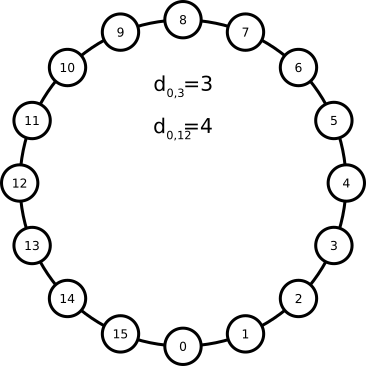
\includegraphics[width=0.75\textwidth]{fig/ring-distance.png}
    \caption{\label{fig:ring-distance}
        \textbf{Left:} Definition of distance $d_{xx'}$ between sites $x$ and $x'$. The distance $d_{xx'}$ is considered on the one
        dimensional chain and does not take into account the connections that determine the coupling.\\
        \textbf{Right:} Example of the initial ring lattice before any rewiring is performed, where the lines represent the coupling
        between units.\\
        One can imagine the dynamics take place on a periodic one dimensional system with interaction range $K$.
    }
\end{figure}

\subsection{Rewiring algorithm}

The rewiring algorithm considers each connection in the starting graph exactly once, and with probability $p$ it tries to swap one of
its vertices for another randomly selected node in the network, avoiding double connections of self connections. Detailed instructions
on how it was implemented are written in pseudo-code bellow.

\noindent
\begin{minipage}{\linewidth}
\begin{lstlisting}
Given a ring lattice with N nodes and range K do:
for z from 1 to K:
    for x from 1 to N:
        with probability p do:
            sample a uniform integer r from 1 to N
            if ( r == x ) or ( connection (x, r) already exists ):
                do nothing
            else:
                remove the connection (x, x+z)
                add the connection (x, r)
\end{lstlisting}
\end{minipage}

To determine the probability the connection $(x, x')$ exists in the rewired graph, we introduce the notion of distance between nodes
$x$ and $x'$. Let this be denoted by $d_{xx'}$, and the distance defined in the one dimensional chain as illustrated in
figure~\ref{fig:ring-distance}. Due to the periodic condition $x \mapsto x+N$ on the boundaries, no distance can be greater than $N/2$,
and thus $d_{xx'}$ is formally defined as:

\begin{align}
    d_{xx'} =
    \begin{cases}
        |x-x'| \quad &\text{if $|x-x'|\leq N/2$} \\
        N-|x-x'| \quad &\text{if $|x-x'| > N/2$}
    \end{cases}
    \label{dist}
\end{align}

To calculate the average values $\left< D_{xx'} \right>$ we consider two cases: $d_{xx'} \leq K$, the \textbf{close case}, and $d_{xx'}
> K$, the \textbf{far case}. The reasoning is that:

\begin{itemize}
    \item If the initial distance between two nodes is less than or equal to $K$, than by construction of the ring graph they start out
        connected. The condition that this connection exists in the final graph is that it was never removed in the first place, or it
        could have been removed and than subsequently reformed.

    \item On the other hand, sites with $d_{xx'}>K$ start out disconnected, and thus a connection $(x,x')$ can only result from one of
        its vertices being rewired that way.
\end{itemize}

With a little deliberation on the rewiring procedure, one will agree that if it produces any connection, it is guaranteed to be present
in the result. Conversely, if it fails to break a connection, that connection is also guaranteed to exist in the final graph.

\subsection{Far case}

\begin{figure}
    \centering
    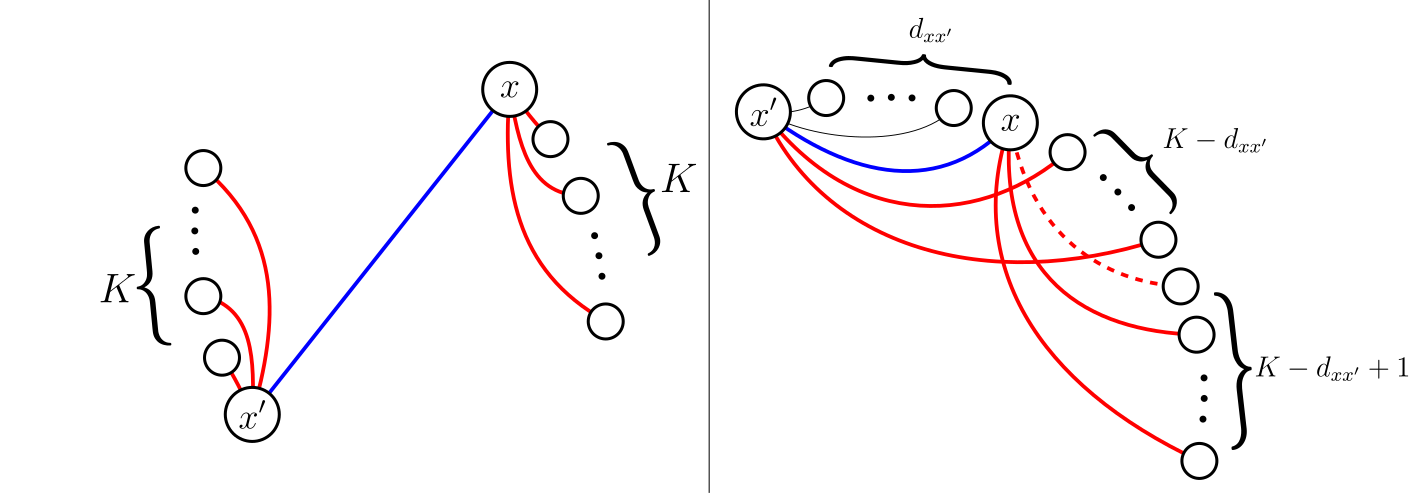
\includegraphics[width=0.9\linewidth]{fig/rewire_contributions.png}
    \caption{The presence of the connection $(x,x')$, in {\color{blue}\textbf{blue}}, in a small-world network generated from the
        Watts-Strogatz algorithm can only be the result of the rewiring of a {\color{red}\textbf{red}} connection. On the left side,
        the \textbf{far} case, $2K$ connections may contribute to the formation of $(x,x')$. On the \textbf{near} case (right side),
        the original connection may either be left untouched or, in the case it is initially broken, it might be wired again by any of
        the remaining $2(K-d_{xx'})+1$ red connections.}
    \label{fig:rewire_contributions}
\end{figure}

Here we derive the probability of existence for a connection between $x$ and $x'$ when $d_{xx'}>K$. Since the algorithm tries to swap
(with probability $p$) the clockwise node of an initial connection, the only connections that could possibly have broken to form
$(x,x')$ are the $K$ clockwise neighbors of $x$, and the $K$ clockwise neighbors of $x'$, as illustrated on the left of
figure~\ref{fig:rewire_contributions}. If any of these $2K$ events take place, $(x,x')$ is guaranteed to exist. Thus, $P(D_{xx'}=1)$ is
the probability that at least one forming event took place, which is just the complement of the probability that \textit{no} such event
took place.

\begin{align}
    P(D_{xx'}=1) = 1 - \left( 1 - \frac{p}{N} \right)^{2K} \qquad \text{for} \quad d_{xx'} > K
    \label{eq:probfar}
\end{align}

In equation~(\ref{eq:probfar}), the probability that a connection rewires to $(x,x')$ is the probability that it breaks times the
probability of selecting the other vertex, which is just $p/N$. Therefore, the probability that a connection \textit{does not} rewire
to $(x,x')$ is the complement $1-p/N$. The probability that \textit{none} of the $2K$ connections generate $(x,x')$ is then
$(1-p/N)^{2K}$, and the probability that at least one of them \textit{does} generate it is the complement again.

\subsection{Near case}

The near case is given by $d_{xx'}\leq K$. When considering the probability of existence for such shorter range connections, things get
more complicated because the exact solutions depend on the choice of the starting point of the rewiring procedure. Consider the case
shown in figure~\ref{fig:order_dependence} for interaction range $K=1$.

\begin{figure}[!ht]
    \centering
    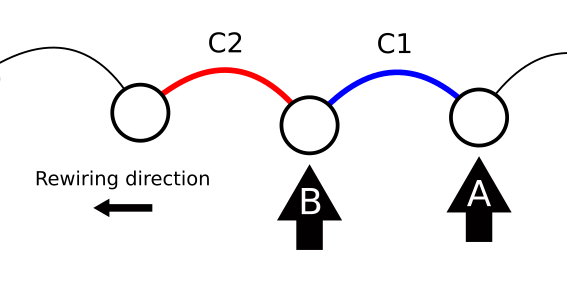
\includegraphics[width=0.7\linewidth]{fig/order_dependence.png}
    \caption{Rewiring of connection C2 may or may not contribute to the probability of existence of connection C1. If the rewiring
    process starts at A, then C2 may be rewired into C1 if it was initially broken. On the other hand, if the starting point is B,
    connection C2 can never be rewired to C1 because the later will always be present at the time of rewiring C2.}

    \label{fig:order_dependence}
\end{figure}

\begin{figure}
    \centering
    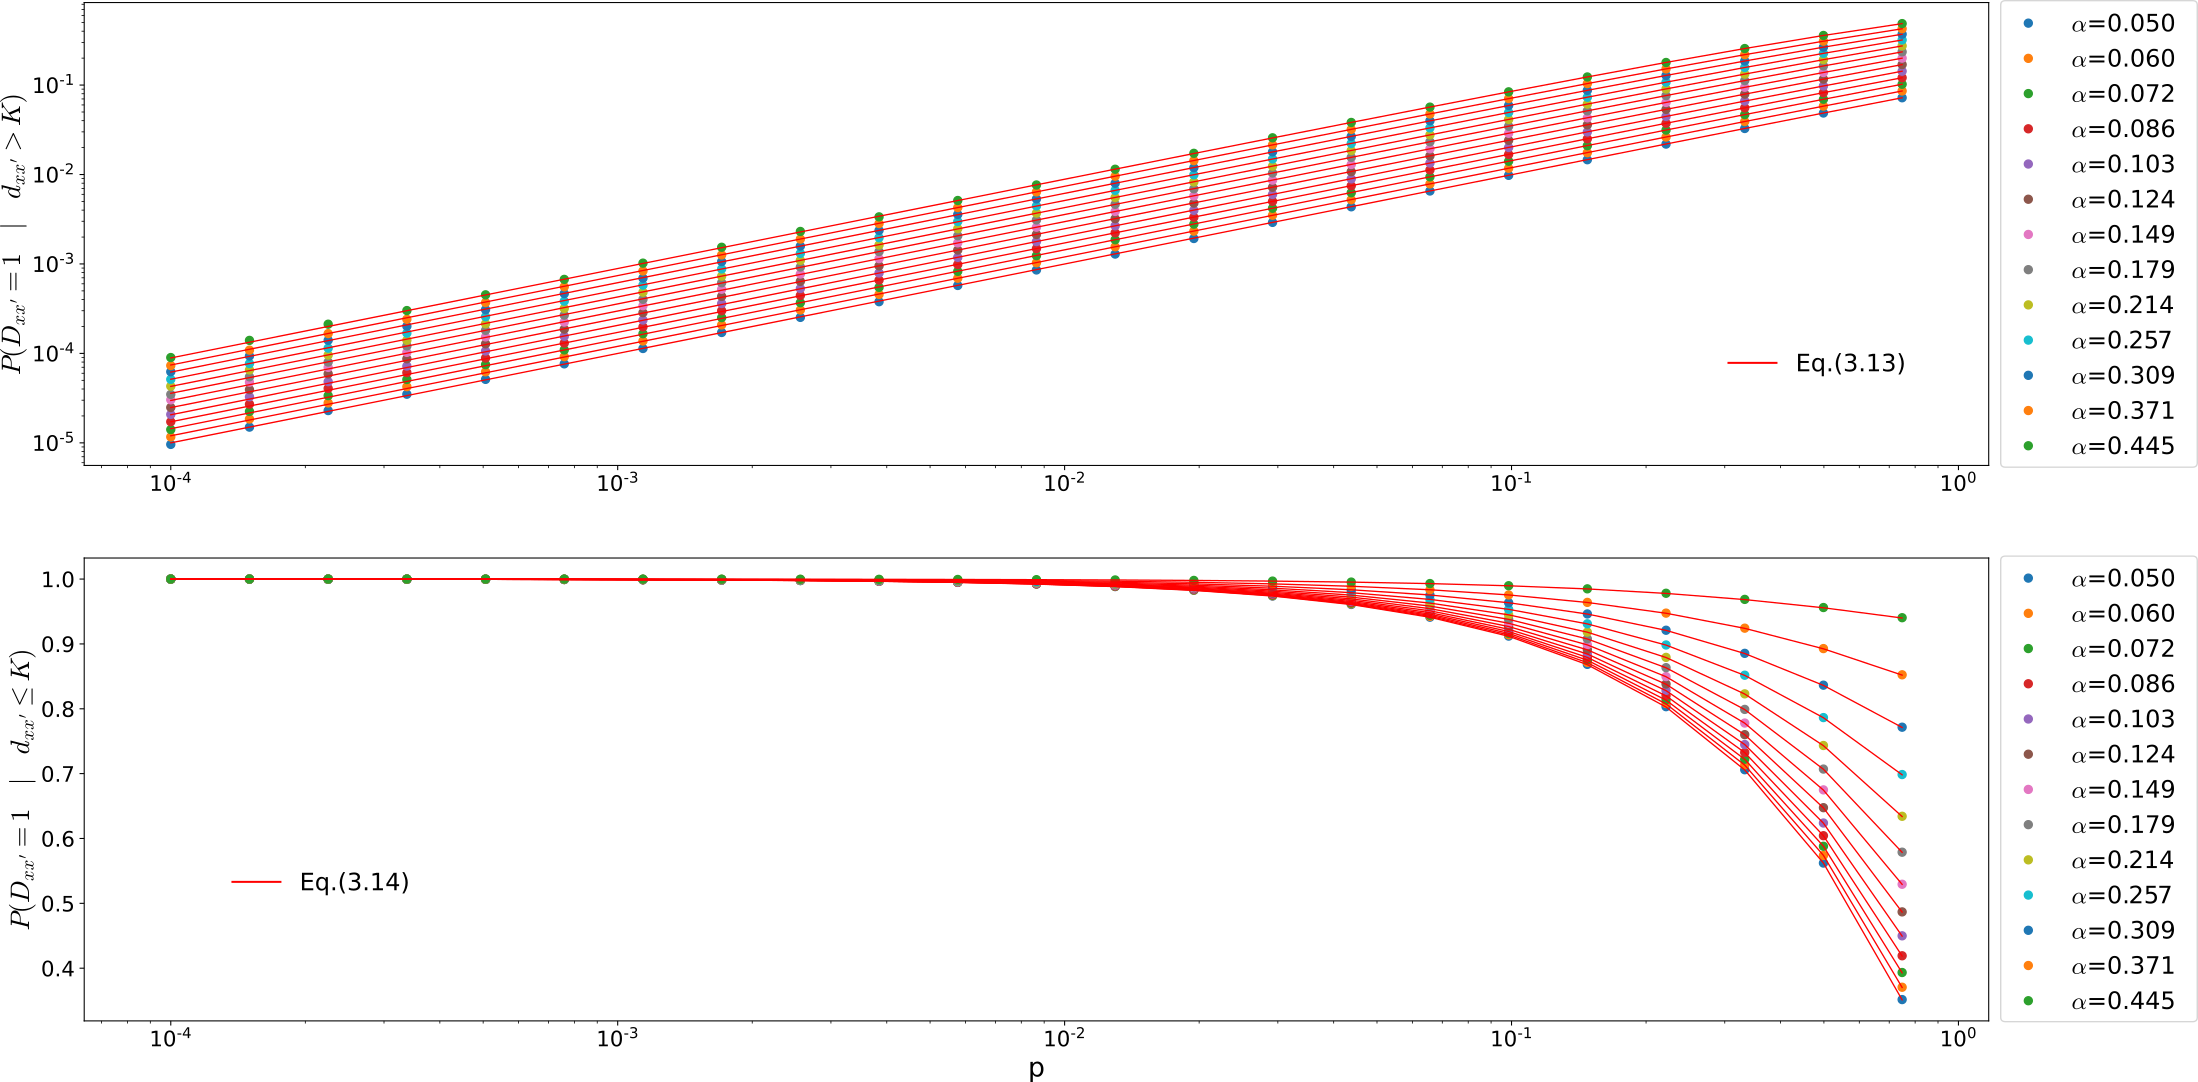
\includegraphics[width=\linewidth]{fig/rewire_mc.png}
    \caption{Comparison between expressions for the probability of existence of connections and those obtained from Monte Carlo
    sampling of small-world networks produced by the Watts-Strogatz algorithm. Size used is $N=1000$ with 50 realizations each.}

    \label{fig:rewire_mc}
\end{figure}

If the rewiring process starts at point A, then rewiring of connection C2 contributes to the probability that C1 is present in the
final graph. On the other hand, if the rewiring starts at point B, then C2 does not contribute to the probability of existence of C1.
Therefore C1 has a higher probability of existing for a rewiring that started at A as opposed to one that started at B. Luckily for our
purposes the order dependence only happens for the first connection of length $d_{xx'}$ (dashed {\color{red}red} line on right of
figure~\ref{fig:rewire_contributions}), since for subsequent connections (solid {\color{red}red} lines on same figure) the pair
$(x,x')$ will already have been considered by the algorithm, and any forming event from that point guarantees the existence of the
connection $(x,x')$.

To avoid order dependence, we will assume the problematic event contributes the same amount as subsequent events to the probability of
existence of the considered connection. Thus, all $2K-2d_{xx'}+1$ events contribute equally to $P(D_{xx'}=1)$, which is written as:

\begin{align}
    P(D_{xx'}=1) = 1 - p\left(1-\frac{2K}{N}\right)\left(1-\frac{p}{N}\right)^{2K - 2d_{xx'} + 1} \qquad \text{for} \quad d_{xx'} \leq K
    \label{eq:probnear}
\end{align}

\noindent As before, the expression is obtained by taking the complement of the probability that no event forms the connection
$(x,x')$: the probability that the original connection is broken is $p(1-2K/N)$ ($p$ times the probability of selecting a site which
does not already have a connection with $x$). This is another approximation since the number of connections involving site $x$ may
change during the rewiring procedure, but because the later conserves the total number of connections it is at least justifiable for
now (we later confirm it through experiment). The term $(1-p/N)^{2K-2d_{xx'}+1}$ accounts for the probabilities that no forming event
occurs with the potential connections marked in {\color{red}red} on the right side of figure~\ref{fig:rewire_contributions}.

\subsection{The discrete average field}

To check that the approximations are valid, we performed Monte Carlo sampling of the small-world networks and plotted the relative
frequencies obtained for the existence of pairs of edges against the probabilities given by equations~(\ref{eq:probfar}) and
(\ref{eq:probnear}). The results are shown, for various values of $p$ and $\alpha \equiv K/N$, in figure~\ref{fig:rewire_mc} where a
good agreement is observed for all values of $p$ and interaction range $K$ for the fixed value of $N=1000$.

Note that we have equated a frequency measure (Monte Carlo sampling) with the associated probability $P(D_{xx'})$ in a frequentist
probability interpretation, and since $D_{xx'}$ are binary variables with values 1 and 0, $\left<D_{xx'}\right> = P(D_{xx'}=1)$,
resulting in

\begin{equation}
    \left<D_{xx'}\right> =
    \begin{cases}
        1-\left( 1 - \frac{p}{N} \right)^{2K} \quad &\text{if} \quad d_{xx'}>K\\
        1-p\left( 1 - \frac{2K}{N} \right)\left( 1 - \frac{p}{N} \right)^{2K-2d_{xx'}+1} \quad &\text{if} \quad d_{xx'}\leq K\\
    \end{cases}
    \label{eq:probconnection}
\end{equation}

Using equation~(\ref{eq:probconnection}) we write the bottom summation of equation (\ref{eq:numf}) as

\begin{align}
    \sum_{x'=1}^N \left< D_{xx'} \right> = &\sum_{d_{xx'}\leq K} \left[
    1 - p\left(1-\frac{2K}{N}\right)\left(1-\frac{p}{N}\right)^{2K - 2d_{xx'} + 1} \right] \notag\\
        + &\sum_{d_{xx'}>K} \left[ 1 - \left( 1 - \frac{p}{N} \right)^{2K} \right]
\end{align}

\noindent which can be expanded into powers of $p$ using the binomial expansion to give

\begin{align}
    \left( a - b \right)^n = \sum_{i=0}^n \binom{n}{i}(-1)^ia^{n-i}b^{i} \notag
\end{align}

\begin{align}
    \label{eq:ppower}
    \begin{split}
    \sum_{x'=1}^N \left< D_{xx'} \right> = \sum_{d_{xx'}\leq K} &\left[ \vphantom{\frac{2K}{N}} \right. 1 - \left( 1 - \frac{2K}{N} \right) p + \frac{\left( 2K-2d_{xx'}+1 \right)}{N} \left( 1 - \frac{2K}{N} \right) p^2 \\
    &- \frac{(2K-d_{xx'}+1)(2K-2d_{xx'})}{2N^2}\left( 1 - \frac{2K}{N} \right)p^3 + \mathcal{O}(p^4) \left. \vphantom{\frac{2K}{N}} \right] \\[12pt]
    +\sum_{d_{xx'}> K} &\left[ 2\frac{K}{N}p - \frac{2K(2K-1)}{2N^2}p^2 + \frac{2K(2K-1)(2K-2)}{6N^3}p^3 - \mathcal{O}(p^4) \right]
    \end{split}
\end{align}

In what follows, we will be interested in the limit of large $N$ while the proportion $K/N\equiv \alpha$ ($\alpha \in \{0, 0.5\}$)
remains \textit{constant}. Therefore we can write the coefficients of $p$ in equation~(\ref{eq:ppower}) as powers of $K$ ($K$ and
$d_{xx'}$) divided by a power of $N$ for the far (near) case. Any terms of the form $K^a/N^b$ with $a<b$ (or of the form
$K^a(d_{xx'})^b/N^c$ with $a+b<c$) will go to zero for large $N$. Retaining only the highest powers for $K$ and $d_{xx'}$ gives:

\begin{align}
    \label{eq:ppower2}
    \begin{split}
    \sum_{x'=1}^N \left< D_{xx'} \right> = \sum_{d_{xx'}\leq K} &\left[ \vphantom{\frac{2K}{N}} \right. 1 - \left( 1 - 2\alpha \right) p + 2\left( \alpha-\alpha_{xx'} \right) \left( 1 - 2\alpha \right) p^2 \\
    &- (2\alpha^2 + \alpha_{xx'}^2 - 3\alpha\alpha_{xx'})\left( 1 - 2\alpha \right)p^3 + \mathcal{O}(p^4) \left. \vphantom{\frac{2K}{N}} \right] \\[12pt]
    +\sum_{d_{xx'}> K} &\left[ 2\alpha p - 2\alpha^2 p^2 + \frac{4}{3}\alpha^3 p^3 - \mathcal{O}(p^4) \right]
    \end{split}
\end{align}

\noindent where we have written $\alpha_{xx'} \equiv d_{xx'}/N$ for brevity.

For small-world networks, the parameter $p$ tends to be small\cite{rodrigues2020synchronization}, as seen from
figure~\ref{fig:small-world}, and considering only terms up to first order in $p$ allows us to perform the summations.

\begin{align}
    \sum_{x'=1}^N \left< D_{xx'} \right> &= \sum_{d_{xx'}\leq K} \left( 1 - p + 2\alpha p \right) + \sum_{d_{xx'}> K} 2\alpha p \notag\\
    &= 2K\left( 1 - p + 2\alpha p \right) + (N-2K)2\alpha p \notag\\
    &= 2K - \cancel{2Kp} + \bcancel{4K\alpha p} + \cancel{2N\alpha p} - \bcancel{4K\alpha p} \notag\\[12pt]
    \sum_{x'=1}^N \left< D_{xx'} \right> &= 2K
    \label{eq:ppower3}
\end{align}

\noindent where we have made use of the fact that $N\alpha = K$. This result is consistent with the previous statement that the average
number of neighbors remains unchanged after the rewiring procedure, and also recovers previous results\cite{escaff2014arrays} for the
case $p=0$.

We now look at the expression $\sum_{x'} \left< D_{xx'} \right> \left< \delta_{jj'} \right>$, the numerator of equation~(\ref{eq:numf})
, where $j$ and $j'$ are the states of oscillators at $x$ and $x'$ respectively. We identify the term $\left< \delta_{jj'}(t) \right>$
with the probability of finding the oscillator at $x'$ in state $j$ at time $t$ and write it as $P^{x'}_j(t)$. The term $\left< D_{xx'}
\right>$ is expanded as before in the limit $N \gg 1$ and $p \approx 0$ and we obtain:

\begin{align}
    \left< \delta_{jj'}(t) \right> &\equiv P_j^{x'}(t) \notag\\
    \left< D_{xx'} \right> &=
    \begin{cases}
        1-(1-2\alpha)p \quad &\text{if $d_{xx'} \leq K$}\\
        2\alpha p \quad &\text{if $d_{xx'} > K$}\\
    \end{cases} \notag\\[12pt]
    \sum_{x'=1}^N \left< D_{xx'} \right> P_j^{x'}(t) &= 2K\alpha p \sum_{d_{xx'}>K}P_j^{x'}(t) + [1-(1-2\alpha)p]\sum_{d_{xx'}\leq K} P_j^{x'}(t)
    \label{eq:numerator}
\end{align}

\noindent by adding and subtracting the sum $2p\alpha\sum_{d_{xx'} \leq K}P^{x'}_j(t)$ to (\ref{eq:numerator}) we can group terms to
obtain

\begin{align}
    \sum_{x'=1}^N \left< D_{xx'} \right> P_j^{x'}(t) &= 2p\frac{K}{N}\sum_{j'=1}^N P^{x'}_j(t) + (1-p)\sum_{d_{jj'} \leq K} P^{x'}_j(t)
    \label{eq:numerator2}
\end{align}

\noindent and finally substituting (\ref{eq:numerator2}) and (\ref{eq:ppower3}) back into equation~(\ref{eq:numf}) gives the MF value
for the parameter $\nu$:

\begin{equation}
    \upsilon_{j,MF}^x(t) = \underbrace{\frac{p}{N}\sum_{x'=1}^N P^{x'}_j(t)}_{\text{Global}}
\quad + \quad \underbrace{\frac{1-p}{2K}\sum_{x'=-K}^K P^{x+x'}_j(t)}_{\text{Local}}
    \label{eq:upsilonp}
\end{equation}

We see that the rewiring process creates a global coupling component while the coupling inside the range $2K$ is reduced by a factor
$(1-p)$. In the limit of $p\to 0$, equation~(\ref{eq:upsilonp}) recovers the MF previously derived by Escaff \textit{et al.} for
regular ring lattices\cite{escaff2014arrays}.

\section{Continuous limit}

In the previous session the discrete MF was derived by taking the limit $N\to\infty$ while keeping the ratio $\alpha\equiv K/N$ fixed.
We now proceed to take the continuous limit of (\ref{eq:upsilonp}) by mapping the oscillator's indexes from 1 to $N$ to the semi-open
interval $[0,1)$ in the reals. The indexes $x,x' \in \{1,...,N\}$ become position coordinates $x,x'\in [0,1)$ and therefore $\nu^x_j(t)
\to \nu_j(x,t)$ where $j$ still represents the state of the unit at $x$ with $j\in\{1,2,3\}$. Analogously, the expression for the
probability of finding the oscillator at $x$ in state $j$ is now $P_j(x,t)$. The periodic conditions for any function of position $x$
becomes $f(x)=f(x+1)$. As for the sums we now have

\begin{align}
    \frac{1}{N}\sum_{x'=1}^N &\to \int_{0}^{1} dx' \notag\\
    \frac{1}{2K}\sum_{x'=-K}^K &\to \frac{1}{2\alpha}\int_{-\alpha}^{\alpha} dx'
\end{align}

\noindent which leads us to the continuous expression for $\nu_j(x,t)$:

\begin{align}
    \nu_j(x,t) = p \int_0^1 P_j(x',t)dx' + \frac{1-p}{2\alpha}\int_{x-\alpha}^{x+\alpha} P_j(x',t)dx'
    \label{eq:numfcontinuous}
\end{align}

\noindent the transition rates from state $j$ to $j+1$ for an oscillator at position $x$ in the continuous MF limit is then given by
rewriting equation~(\ref{eq:mfrate}) with the notation $\gamma^x_j(t) \to \gamma_j(x,t)$ and using (\ref{eq:numfcontinuous}) in place
of $\nu^x_j$:

\begin{align}
    \gamma_j(x,t) = g(x) \exp\left[ a\left( \nu_{j+1}(x,t) - \nu_j(x,t) \right) \right]
    \label{eq:ratecontinuous}
\end{align}

\noindent where $g(x)$ is the uncoupled frequency of the oscillator at $x$, sampled from some unimodal symmetric distribution.

The set of $2N$ master equations (\ref{eq:motion}) that describe the time evolution of probabilities reduce to just 2 equations for the
now spatially distributed probability $P_j(x,t)$. Again we have the condition $P_1(x,t) + P_2(x,t) + P_3(x,t)=1$ so that we only need
two equations to describe the probabilities of all three states.

\begin{align}
    \ddt{P_1}(x,t) &= \gamma_3(x,t)\left(1-P_1(x,t)-P_2(x,t)\right) - \gamma_1(x,t)P_1(x,t) & \notag\\
    \ddt{P_2}(x,t) &= \gamma_1(x,t)P_1(x,t) - \gamma_2(x,t)P_2(x,t) & x\in[0,1)
    \label{eq:motioncontinuous}
\end{align}

The solutions of equations~(\ref{eq:motioncontinuous}) thus describe the predicted behaviors of sufficiently large populations of
oscillators, and can be compared to direct simulations of the dynamics.

\section{Solutions for the continuous mean field}

The system described by equations~(\ref{eq:ratecontinuous})~and~(\ref{eq:motioncontinuous}) is the MF approximation for the rewired
ring lattices. One solution to this sytem is $P_1(x,t)=P_2(x,t)=1/3$, called the \textit{quiescent} solution. To see this, not that
from equation~(\ref{eq:numfcontinuous}) we have $\nu_1(x,t) = \nu_2(x,t)$ when the probabilities are the same, and therefore

$$\gamma_1(x,t) = \gamma_2(x,t) = \gamma_3(x,t)=g(x)$$

\noindent from equation~(\ref{eq:ratecontinuous}). The \textit{quiescent} solution is stable when the coupling strength $a$ is bellow
some critical value $a_c$ that depends on the couplings and whose lowest value is attained for the complete graph, with $a_c=1.5$. The
threshold $a_c$ marks a Hopf bifurcation\footnotemark type transition for graphs that support global
oscillations\cite{Wood06a}\cite{rodrigues2020synchronization}\cite{Wood06b}\cite{Wood07b}. When the coupling $a$ is larger than the
critical value $a_c$ the \textit{quiescent} solution becomes unstable and self-organization takes place, usually in the form of global
synchronization. This does not necessarily mean global oscillations are stable in the mathematical sense. Analysis for the globally
synchronized phases has been notoriously difficult for oscillator models in general.

\footnotetext{A Hopf bifurcation occurs when a periodic solution arises around an equilibrium point as some parameter varies. Here, the
oscillations arise around the \textit{quiescent} solution as $a$ increases past $a_c$.}

In chapter~\ref{chap:4} we explore simulations on small-world networks with strong coupling that do not always lead to global
oscillations. Depending on initial conditions and the inherent noise the system may converge to a travelling wave solution, displaying
only local synchronization. Following a similar analysis by Escaff et al.\cite{escaff2014arrays} we investigate such a wave solution by
perturbing the \textit{quiescent} state with a waveform and then checking what happens to the time evolution of the amplitude of said
perturbation, which we modulate by some arbitrary parameter $\epsilon_j$:

\begin{align}
    P_j(x,t) = 1/3 + \epsilon_j e^{ikx + \lambda t}
\end{align}

\noindent where $i=\sqrt{-1}$, and $k\in\mathbb{R}$ and $\lambda\in\mathbb{C}$ are the spatial and temporal angular frequencies of the
wave respectively.  Assuming the perturbed solution is still a solution to the master equations~(\ref{eq:motioncontinuous}), the goal
is to identify whether there are any conditions on the model parameters that allow for $\operatorname{Re}[\lambda]>0$, since in such
case the amplitude of the waveform would increase as $t$ grows. Thus, for wave solutions we have

\begin{align}
    \ddt{P}_j(x,t) &= \lambda e^{ikx + \lambda t} \\[12pt]
    \nu_j(x,t) &= \frac{p}{3} + pe^{\lambda t}\int_0^1 e^{ikx'} dx' + \frac{1-p}{3}
\end{align}
